\documentclass[conference]{IEEEtran}
\IEEEoverridecommandlockouts
% The preceding line is only needed to identify funding in the first footnote. If that is unneeded, please comment it out.
\usepackage{cite}
\usepackage{amsmath,amssymb,amsfonts}
\usepackage{algorithmic}
\usepackage{graphicx}
\usepackage{textcomp}
\usepackage{xcolor}
\usepackage{mathtools} 
\usepackage{fixltx2e}
\usepackage{blindtext}
\usepackage{gensymb}
\usepackage[compact]{titlesec}        
% \titlespacing{\section}{0pt}{0pt}{0pt} 
%\AtBeginDocument{%                    
%  \setlength\abovedisplayskip{0pt}
%  \setlength\belowdisplayskip{0pt}}
\usepackage[rawfloats=true]{floatrow} 
\restylefloat{figure}  
\def\BibTeX{{\rm B\kern-.05em{\sc i\kern-.025em b}\kern-.08em
    T\kern-.1667em\lower.7ex\hbox{E}\kern-.125emX}}
\begin{document}

\title{Study of Rapid Charging in Mobile Devices}

\author{\IEEEauthorblockN{Raj Joshi}
\IEEEauthorblockA{\textit{Master Seminar Thesis, SoSe 2019,} 
\textit{University of Bamberg,}
Germany \\
joshiraj008@gmail.com}

}

\maketitle
\thispagestyle{plain}
\pagestyle{plain}

\begin{abstract}

Smartphone users always tend to demand extended battery
availability in their battery use. Along with large battery capacity, fast
charging also helps improve user experience in battery use. There are
various fast charging techniques developed by the OEMs of many devices.
However, the existing techniques lowers the charging speed while the
smartphone is in use. The degradation of charge speed occurs due to the
heat generation caused because of device usage. In this thesis, we compare
existing fast charge schemes with an adaptive charging scheme called
WARP Charge 30 by OnePlus, which enables rapid charging of battery
even when device is in use. The main focus of this charging scheme is to
make sure that heat generation does not affect the charging speed
performance and activities running on the smartphone. This charging
scheme is implemented in smartphone models like OnePlus 6T McLaren, 7
and 7Pro. The experimental demonstration via various sources and claims shows that
the charging speed of this scheme is up to 38\% faster as compared to other
schemes, while preserving device performance.

\end{abstract}

\begin{IEEEkeywords}
mobile devices, fast charging, battery lifetime
\end{IEEEkeywords}

\section{Introduction}

Mobile devices consume a large amount of energy therefore users experience situations where the battery does not last more than a day. Users have to charge their devices several times a day and sometimes even carry an extra brick of battery or a portable power-bank. To solve this, device manufacturers have
been offering fast charging technologies, such as Quick Charge\cite{b4}, Adaptive Fast Charging\cite{b5} and DASH Charging\cite{b6}. One Plus's Dash Charging is, for example has reported to charge 63\% of the OnePlus 3's 3000 mAh battery within 30 min. Even though the fast charging technology helps users cope with their battery problem, mobile users often use their devices aggressively, for example, playing heavily loaded 3D games. The power demand is so high that some users even carry a phone holder to charge the battery while using the device.   

Recently, it was observed in a situation where the charging speed slows down especially when the device is in use. This issue has not been reported in previous studies or related documents\cite{b7}-[10]. In the preliminary observations it was seen that the existing charging method exercised in commercial devices reduces the charging power excessively when the device is in use. This phenomenon was analyzed and based on understanding of the charging path in mobile devices, it was found that this is caused by the device manufacturer’s specific charging control which charges the device with a fixed power. In general, the charging power of a mobile device is controlled to prevent performance degradation caused by the temperature rise of the device\cite{b11,b12}. However, since the charging power is controlled without information about the device usage, charging is conducted inefficiently. This inefficiency slows down the charging speed even when the device screen is only turned on and with no applications or services running on top of it.     

In this Thesis, we discuss and address the inefficiency of the existing charging methods, also compare it with many parameters defined. The focus will be on WARP charge 30 industrial standard charging scheme and it's possible drawbacks.   

\section{Evolution of Fast Charging}

\subsection{Qualcomm's Quick Charge}

Qualcomm’s has a default proprietary charging scheme known as Quick Charge, as it popularized fast charging before USB Power Delivery. The latest version of Quick Charge (v4.0+) is compatible with Power Delivery, allowing faster-charging speeds and a wide range of support. 

\begin{figure}[h!]
  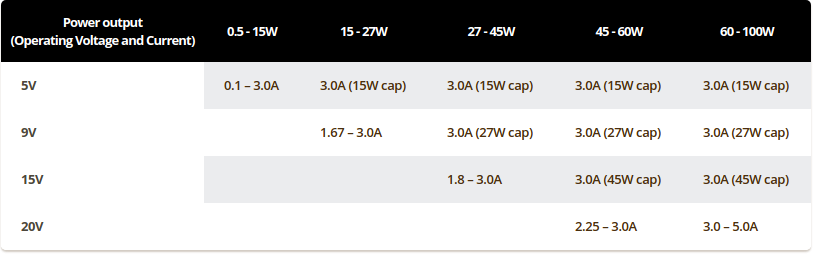
\includegraphics[width=\linewidth]{images/image1.png}
  \caption{Quick Charge versions and output\cite{b13}}
\end{figure}

In Fig.1 above, we can see the evolution of different Quick Charge versions and also observe the improvements over the time in terms of Voltages, Max Current and Max Power respectively.

Quick Charge technology is an optional feature available with Qualcomm's Snapdragon processors. So just because a phone has a Snapdragon chip does not make it Quick Charge compatible. However, a wide range of phones has Quick Charge support, including the LG V40, Xiaomi's Mi 8, Samsung Galaxy Note 9, HTC U12 Plus, etc. There is also a broad availability of legacy chargers and third-party accessories out there, due to its popularity.

\subsection{Other Standards}

In the smartphone ecosystem, many OEMs use their own standards rather than more ubiquitous standards above. Only a few of these standards are truly proprietary. Many of them are just Power Delivery or Quick Charge repackaged under a branding or featuring some specific tweaks to the technology such as Samsung’s Adaptive Charging and Motorola’s Turbo Charging technologies.

Others like Oppo's VOOC and Huawei's SuperCharge function differently. These tremendously increase the amount of current for high power charging rather than increasing the voltage. The charging speeds of these proprietary technologies have greatly increased over the years, with SuperCharge, Super VOCC, and OnePlus WARP Charge 30 being some of the fastest in the modern market. Here is how some of the most common technologies perform up side by side. 

\begin{figure}[h!]
  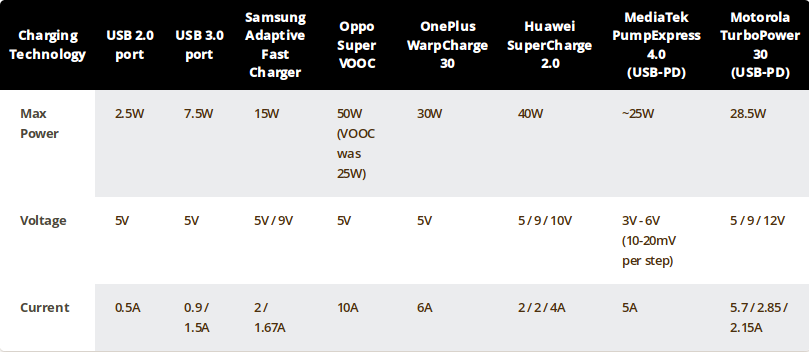
\includegraphics[width=\linewidth]{images/image2.png}
  \caption{Comparison with maximum Power, Voltage and Current alongside various technologies\cite{b13}}
\end{figure}

Above Fig.2 shows us various industry standards stacking side by side with different parameters such as max Power, Voltage and Current. It is observed how various standards modify their parameters in order to make tweaked charging systems. 

\subsection{Testing with various combinations of equipment on different smartphones.}

It is possible to support multiple standards or maybe ensure some level of compatibility with different fast charging methods. Unfortunately, this produces a lot of unpredictability about the accurate charging speeds you will receive when using phones with different chargers and even different cables respectively.

\begin{figure}[h!]
  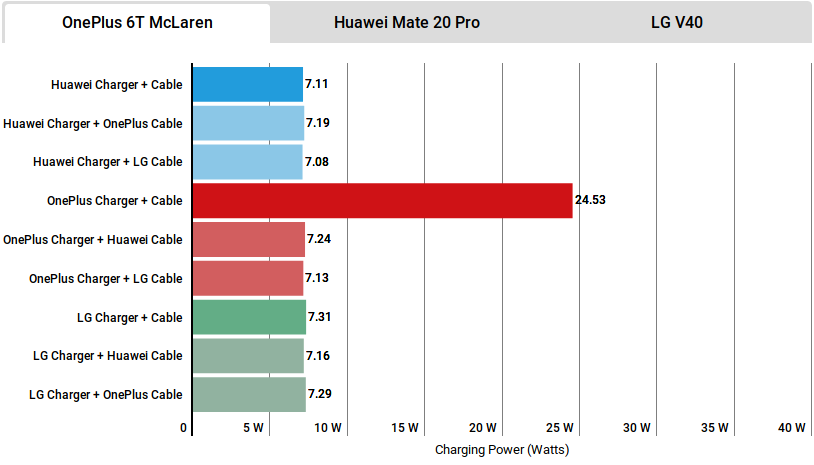
\includegraphics[width=\linewidth]{images/image3.png}
  \caption{OnePLus 6T McLaren\cite{b13}}
\end{figure}


In the above Fig.3, the change in Charging Power (Watts) is clearly observed when a specific charger is applied, in this case it is OnePlus official bundled charger which comes along with the device. This proves the fact that different chargers or cables are not accurately compatible with underlying charging scheme used by the device.

\begin{figure}[h!]
  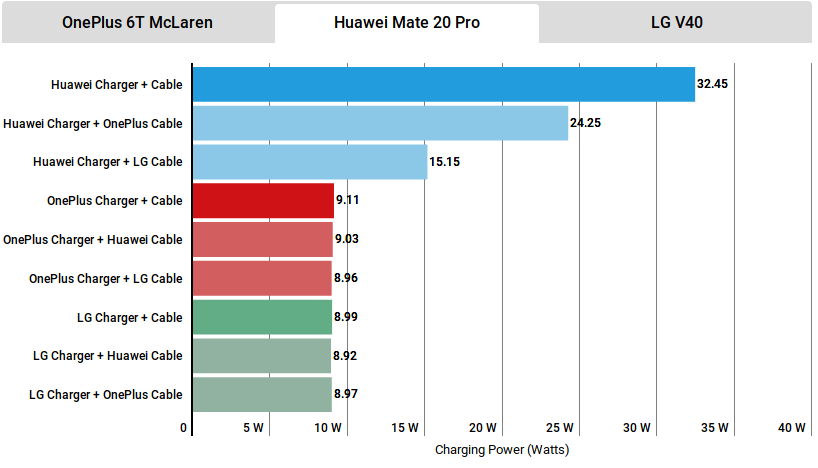
\includegraphics[width=\linewidth]{images/image4.png}
  \caption{Huawei Mate 20 Pro\cite{b13}}
\end{figure}


Fig.4 shows that when the combination Huawei charger and gives a max Charging Power of 32.45W with its official bundled charger-cable combination while on the other hand it is performing acceptable in terms of Charging Power with Huawei charger-OnePlus cable, however when connected to rest equipment it fails to deliver the same speeds. This again proves the fact that different chargers or cables are not accurately compatible with underlying charging scheme used by the device.  

\begin{figure}[h!]
  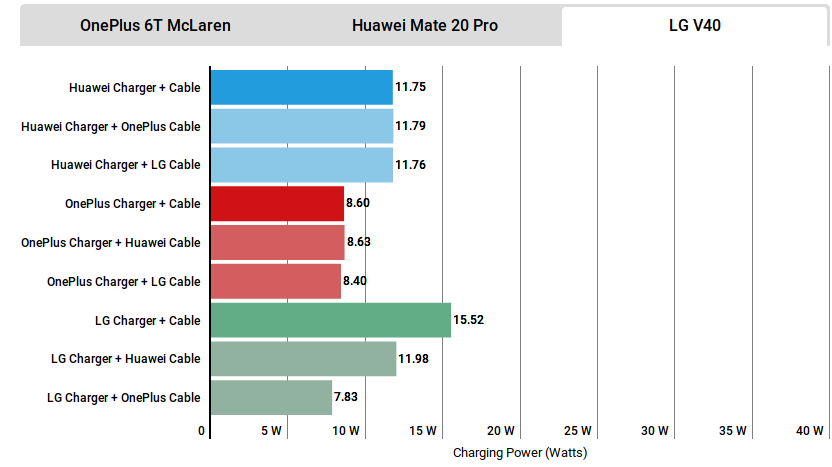
\includegraphics[width=\linewidth]{images/image5.png}
  \caption{LG V40\cite{b13}}
\end{figure}


In Fig.5 it is observed that LG charger+Cable combination charges at 15.52W while the others lack the same consistent speeds and are not up to the original charging power. So again we can conclude that other OEM charger or cable combination will not work accurately well. 

After testing several phones, it was found that a wide variation in how much power each phone faired, depending on the charger and cable used. The best results are typically achieved by using the cable and charger supplied in the box with your handset.

\subsection{Charging Speed while Using Device}

\begin{figure}[h!]
  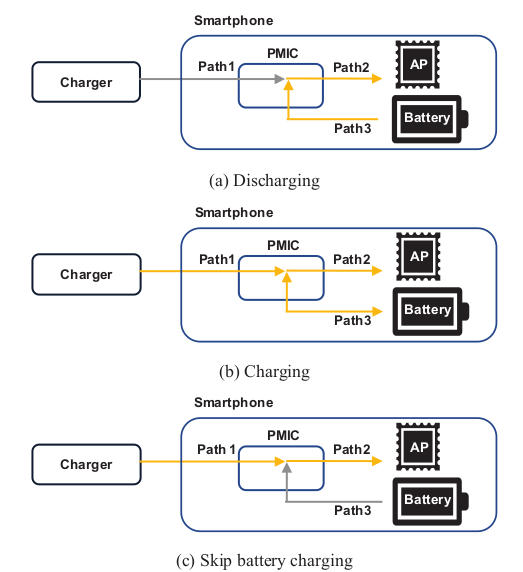
\includegraphics[width=\linewidth]{images/image6.png}
  \caption{Current Charging Paths inside a Smartphone\cite{b1}}
\end{figure}

To get an idea about how a smartphone is charged, the author\cite{b1} identified the hardware parts in mobile devices. Fig.6 depicts the current paths of typical smartphones where the yellow line is for the current flow. When the phone is discharged without charging (Fig. 6(a)), the PMIC (Power Management Integrated Circuit) draws current from the battery via Path3 and provides it to the application processor (AP) through Path2. When charging proceeds, the power from the external charger flows into the PMIC through Path1. The external power is then consumed by the AP via Path2, while the residual power is flown into the battery through Path3 (Fig. 1(b)). When the kernel blocks battery charging in the case of a full charge, the PMIC does not charge the battery and provides current directly to the AP via Path2 (Fig. 6(c)). \cite{b1}

Modern Smartphones tend to charge faster when the screen is turned off and when there is no system load or severe power consuming services running in the background. However, as the screen is turned on, the charging power decreases immediately. This reduced power is then maintained at the same level while the screen is on. This charging behaviour is not efficient because the status of charging is not immediately changed when screen is turned on. As the author \cite{b1} mentioned in their thesis that the device was doing nothing while the screen was on, consuming less than 2 W; therefore, an additional 5 W of power could have been used for charging in this case.\cite{b1}

\subsection{Charging Speed vs Performance}

As we mention charging speed reduction in the previous section, it is hypothesised in document \cite{b1} that charging increases device temperature drastically. Hence, to control this phenomenon the operating system aggressively cuts the charging power which in turn results into slower charging rate. In general, heat affects the performance of a mobile device. When the AP’s temperature peaks a certain point, the kernel starts to throttles the device’s performance to a lower temperature resulting decreased performance. Most of the tests done were based on FPS (frames per second) metric. This is because the smoothness of the display is crucial part of User experience. The lags or jitters occurring during running applications or games play a major part of normal usage of a smartphone user. It was also observed that performance degradation happened due to thermal throttling of GPU (Graphics Processing Unit) in smartphone as mentioned by the author in document \cite{b1}.    

To conclude this study, it was observed that the temperature of the PMIC component in the device increases during charging, and the heat generated by the PMIC affects the AP. As a result, charging raises the temperature of the AP. Eventually, the heat generated by charging affects the performance of the device
in some cases, when a heavy workload is running. Also, the default charging mechanisms implemented in commercial devices are inefficient, especially when the device is in use. 

\section{DASH Charge}

DASH Charge technology is a licensed version based on VOOC 2.0 (Voltage Open Loop Multi-step Constant-Current Charging)\cite{b14} which is rebranded by the Chinese smartphone company One Plus. It is a proprietary rapid-charging technology created by OPPO Electronics which can charge supported devices from 0-63\% in just 30 minutes without hindering device performance which has been claimed by the OEM. \cite{b6}  However, the study in this thesis will not be just based on the claims of the company rather it will give insight into this standard and show How is this charging scheme better than the existing ones.

As it was seen previously, Quick Charge 1.0 only allowed for 2 AMPs at 5V for 10 watts of power and most chargers these days come close to this specification. Older chargers operate at 5 volts and put out little more than 1 amp of current, if not less. Rather than just scaling up the voltages for more power and a smaller transfer drop, Dash Charge aims to brute force more current over 5V. The standard peaks at 5 AMPs, allowing for a massive 25 W of power to charge the battery with, in ideal operating conditions. That’s a 66\% increase in power over Quick Charge 2.0 and explains why Dash Charge technology appears that much faster. With raw power, there are also some subtle differences between the ways each design detects compatible smartphones. Qualcomm’s charger design matches the maximum power output to the device voltage, leaving the phone's internal circuitry to draw the correct amount of current and dissipate the heat. 

\begin{figure}[h!]
  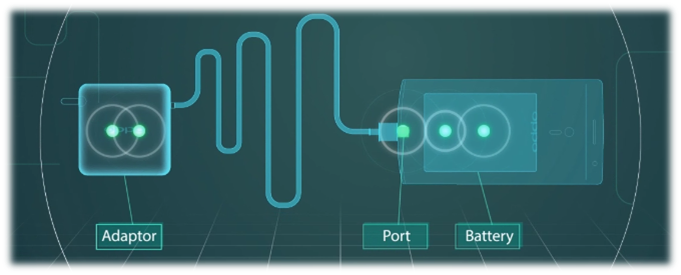
\includegraphics[width=\linewidth]{images/image7.png}
  \caption{Dash Charge/VOOC 2.0 Charge Circuit Design\cite{b15}}
\end{figure}



In the above Fig.7, we can see the highlights marked with bright circular nodes as the power input, output, recipient port and battery respectively. OnePlus has moved the current control circuit to the charger itself, resulting in less heat dissipation in the handset, which is good for component lifespans. The charger is able to detect whether or not the device is Dash compatible, and will supply the correct current, either 5A or 1A, to the device to prevent damage. The trade-off here is a lack of flexibility with other products; you can’t optimally charge a 3 AMPs Quick Charge 2.0 phone with the Dash adaptor for example, but a Quick Charge 2.0 adaptor is backwards compatible with handsets that don’t quite meet its maximum specifications\cite{b15}.

Now the question arises if it is hardware enabled then what is the architecture underlying the cable look like. To uncover this, there was a cable tear-down test taken by one of the users\cite{b16}.

\begin{figure}[h!]
  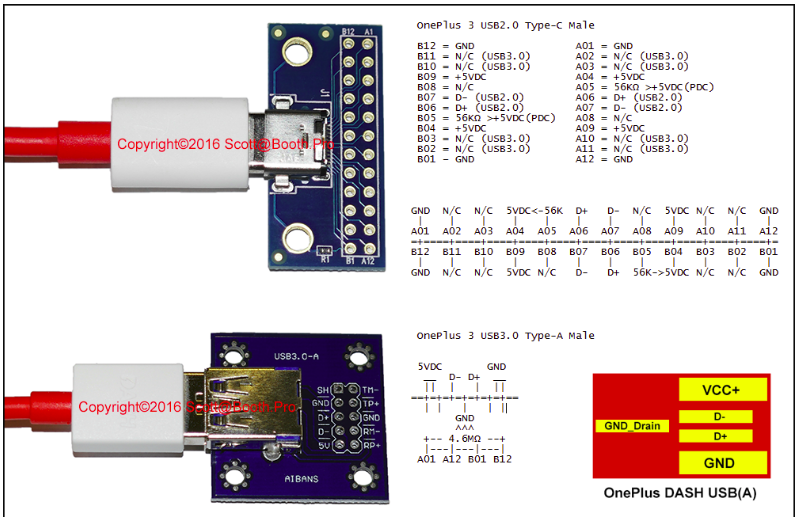
\includegraphics[width=\linewidth]{images/image8}
  \caption{Underlying Cable Architecture\cite{b16}}
\end{figure}

Fig.8 illustrates us the pin connection structure inside the cable connector. There were findings as well such as the USB3.0 TX/RX pins are missing except for the rear GND\_Drain pin, which is thought to be having something to do with the DASH feature. It was understood that, there is a 56K resistor tied between the +5VDC and the PDC [Power Data Communication] pin next to it.\cite{b16} And there is an interesting low resistance (4.6M ohm) tie-in between the GND\_Drain pin and the other primary GND pins; like something is in-circuit facilitating a feature trigger(DASH).

\section{Related Work}

\subsection{Always on Quick Charging}

Always on Quick Charging (AQC), is a custom charging scheme implemented by the author in \cite{b1}. This scheme controls the charging rate in order to provide a fast charging speed even with device use. The key idea is to maintain the maximum charging power without performance degradation caused by heat generated along with charging. 

One of the main challenges is to accurately predict the performance degradation due to the heat, and to figure out the effect of regulating the charging rate on a mobile device. The authors \cite{b1} focused on thermal throttling which degrades the performance of the device resulting from the increase in temperature.
The thermal throttling works based on two parameters: the thermal threshold, T\textsubscript{threshold} and the clearing set point, T\textsubscript{clr}. T\textsubscript{threshold}is the temperature point at which the throttling should be activated, whereas T\textsubscript{clr} is the target temperature at which the temperature is to be lowered. Thermal throttling occurs when the temperature reaches T\textsubscript{threshold} and is released when the temperature reaches T\textsubscript{clr}. When the AP temperature reaches T\textsubscript{threshold} and performance degradation is expected, the proposed scheme lowers the charging power drastically to decrease the temperature immediately. When the AP temperature drops below T\textsubscript{clr}, the charging power is raised slowly until the AP’s temperature becomes higher than T\textsubscript{clr}. The charging power is maintained while the AP temperature stays between T\textsubscript{threshold} and T\textsubscript{clr}. That is, the charging power is increased up to the point where the thermal violation does not occur. \cite{b1}

\begin{figure}[h!]
  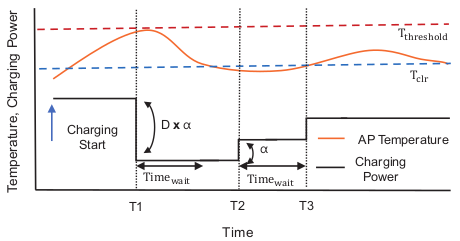
\includegraphics[width=\linewidth]{images/image9.png}
  \caption{Concept of Always-on Quick Charging\cite{b1}}
\end{figure}

In general Fig.9 illustrates the working mechanism of the scheme, when the charging starts, the charging power is kept at the maximum. As the charge advances, the temperature is checked to see if it has reached T\textsubscript{threshold}. If it has, the charging rate is decreased by D (T1 in the figure). After waiting Time\textsubscript{wait}, if the temperature is lower than  T\textsubscript{clr}, the charging power is increased by $\alpha$ (T2). Gradually, if the temperature stays between T\textsubscript{threshold} and T\textsubscript{clr}, the charging rate is maintained (after T3). This way, AQC implements the charging power without a thermal violation. Compared to previous studies\cite{b7}-[10], \cite{b1} is the first to handle the issue on increasing charging efficiency in mobile device. 

Always-on Quick Charging is implemented on Google’s Pixel 2XL smartphone running Android 8.1.0 (Oreo). The author modified the kernel to regulate the charging power and monitor the temperature. Because AQC requires modifications of only the kernel, the scheme can be applied to other mobile devices that support quick charging. In Pixel 2XL, the charging current can be controlled by modifying the PMIC driver. They adjusted the charging rate by changing the POWER\_SUPPLY\_PROP\_CONSTANT\_CHARG\_CURRENT
\_MAX value in /driver/power/*smbcharger.c which determines the charging current. Note that controlling the charging current is enabled if the charger and the device support fast charging. To monitor the device temperature, they collected data from /sys/class/thermal/. We obtained various information, such as the list of temperature sensors and the temperature data of other modules, including the AP, battery, and cameras.Finally, the actual charging control is conducted by an application. We developed an application that monitors the AP temperature in the background and controls the charging using the kernel interface.

\begin{figure}[h!]
  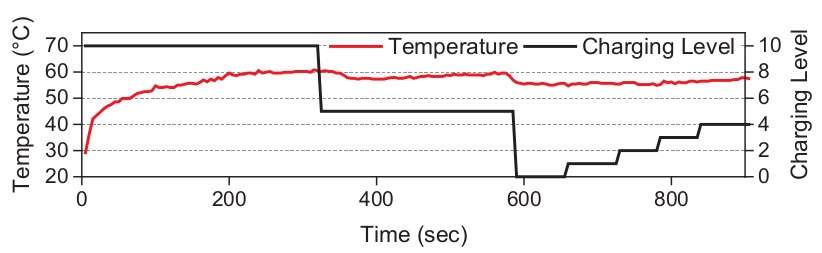
\includegraphics[width=\linewidth]{images/image10.png}
  \caption{AQC performance with thermal workload\cite{b1}}
\end{figure}

To further analyze the detailed operation of the AQC, the author\cite{b1} observed the charging level and temperature specifically with thermal workload. Fig.10 depicts the charging level was the maximum at the beginning of the experiment because the temperature was much lower than T\textsubscript{clr}. Around 300 s, the temperature reached a thermal violation point, and the charging level dropped to 5, which results in decreasing temperature. As the temperature stayed between T\textsubscript{violation} and
T\textsubscript{clr}, the charging level remained at 5. When the temperature rose to T\textsubscript{violation} at around 600 s, the proposed scheme dropped the charging level again. After waiting 60 s, the charging level increased by one because the temperature was under T\textsubscript{clr}. Finally, the proposed scheme determined the optimal charging level was 4. \cite{b1}

\begin{figure}[h!]
  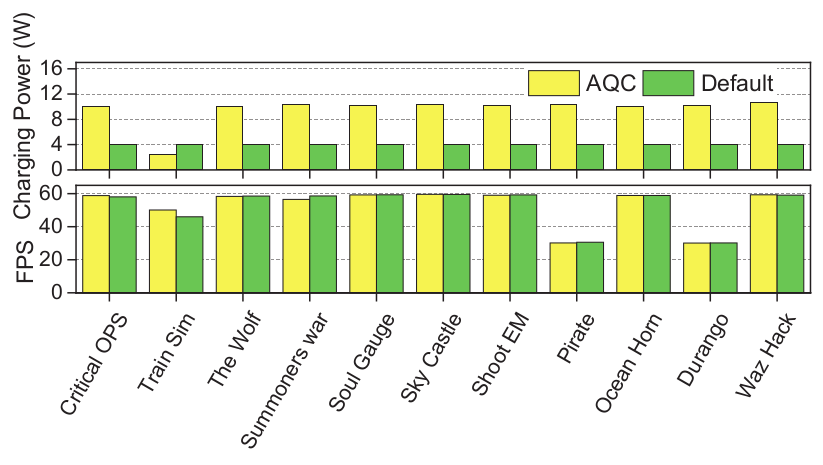
\includegraphics[width=\linewidth]{images/image11.png}
  \caption{Performance with real applications\cite{b1}}
\end{figure}

The author \cite{b1} then validated the effectiveness of the AQC with real applications whose workload changed dynamically. We measured the power consumption and the FPS while running the applications in Fig. 9, for 15 min. In Fig. 11, the charging power and the FPS of the proposed system are compared with those of
the baseline system. For all applications except for Train Sim, AQC improved the charging efficiency by 2.4 times compared to the default charging system while preserving the FPS with only a 3\% loss. In the case of Train Sim, AQC lowered the charging current to guarantee the FPS because a large amount of heat was generated due to the high workload. Consequently, although the FPS of both systems was under 60, the FPS of the proposed system was higher than that of the baseline. Note that the user’s quality of experience for Pirate and Durango was not degraded because their maximum FPS was 30.

\begin{figure}[h!]
  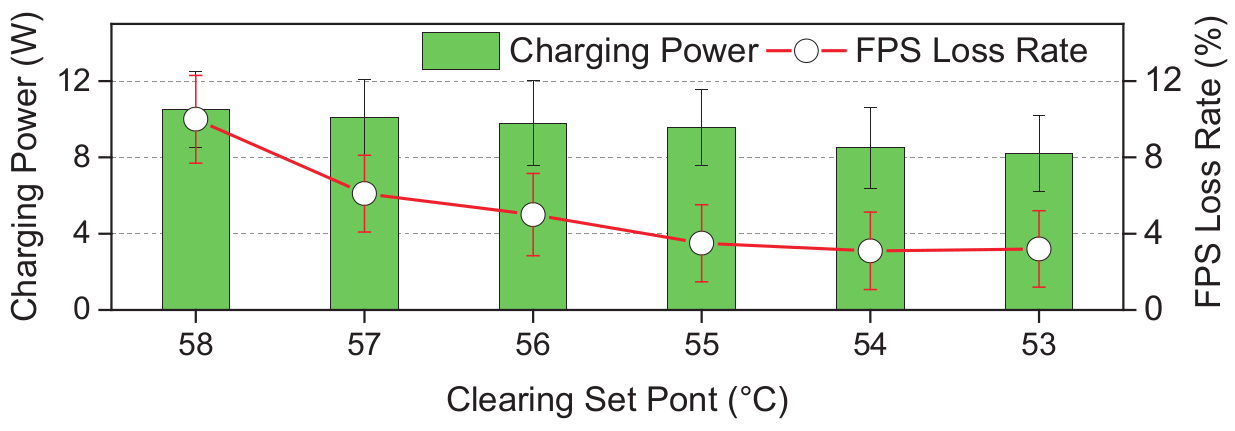
\includegraphics[width=\linewidth]{images/image12.png}
  \caption{Charging power and FPS loss vs. clearing set points\cite{b1}}
\end{figure}

AQC has two critical parameters:the number of charging steps L and the clearing set point T\textsubscript{clr}. In the evaluation, author\cite{b1} determined the number of charging steps heuristically. As other parameters such as $\alpha$, T\textsubscript{$\alpha$} and D are
calculated by L, it severely affects the performance of the proposed scheme. It was observed that the charging efficiency and FPS had loss according to L. However, because the charging power for one step
is large, the temperature increased sharply although the proposed system raised only a single step. Therefore, thermal throttling occurred more often, degrading the FPS. However,
when the charging level was more finely divided, the FPS was preserved, but the average charging power decreased because the charging level increased too slowly. Following this principle, ten steps of charging were chosen for the target device Pixel 2XL.

In the case of T\textsubscript{clr}, the value was set at 55$\degree$C he same as for the baseline system. Because the existing charging system aims to preserve the user experience rather than the charging efficiency, author\cite{b1} consider 55$\degree$C a conservative threshold. It was specifically measured as charging power and the FPS according to T\textsubscript{clr} Fig. 12 indicates that as T\textsubscript{clr}increases, the charging speed becomes faster because the charging level is raised up until the temperature reaches T\textsubscript{clr}. However, thermal throttling occurred more frequently, degrading the FPS. As the ultimate goal of AQC is maximizing the charging efficiency without FPS loss, 55$\degree$C is chosen as appropriate for Pixel 2XL. Note that these results would change depending on the target device\cite{b1}.

In summary, the experiment results verified that Always-on Quick Charging outperforms the original charging system in terms of charging efficiency and FPS. By balancing the charging current and temperature increment, AQC maximized the charging efficiency while preserving the FPS. Although the user experience of a high-workload application was degraded, the proposed system still provided a high FPS, compared to the
original system, by aggressively lowering the charging current.

\section{WARP}

WARP charging is based on improved version of Super VOOC which we discussed in Section III. It is given a standard version of VOOC 3.0 and licensed to OnePlus. The company introduced this standard in 2018 and
quotes charging speeds going from flat to 50\% in just 20 minutes. This is noticeably much faster than DASH charge. 

While there are other fast charging solutions that let you top up your battery quickly, the advantage with OnePlus' implementation is that it doesn't overheat your phone. That's because most of the charging circuitry is offloaded onto the wall unit and is different from the majority of quick charging options
available today\cite{b17}. OnePlus uses dedicated circuitry in the charger itself for heat management and dissipation, which is why you can only get Warp Charge speeds with OnePlus-branded wall and car chargers — such as the one that's included in the OnePlus 7 Pro's box. The key difference between the two fast charging technologies is that while Qualcomm uses higher voltages to charge batteries, VOOC relies on delivering a higher amperage. For instance, Quick Charge 3.0 goes up to 6.5V at 3A, creating 19.5W, whereas Warp Charge delivers 5V at 6A to attain 30W. And that has a few advantages\cite{b17}. 

\begin{figure}[h!]
  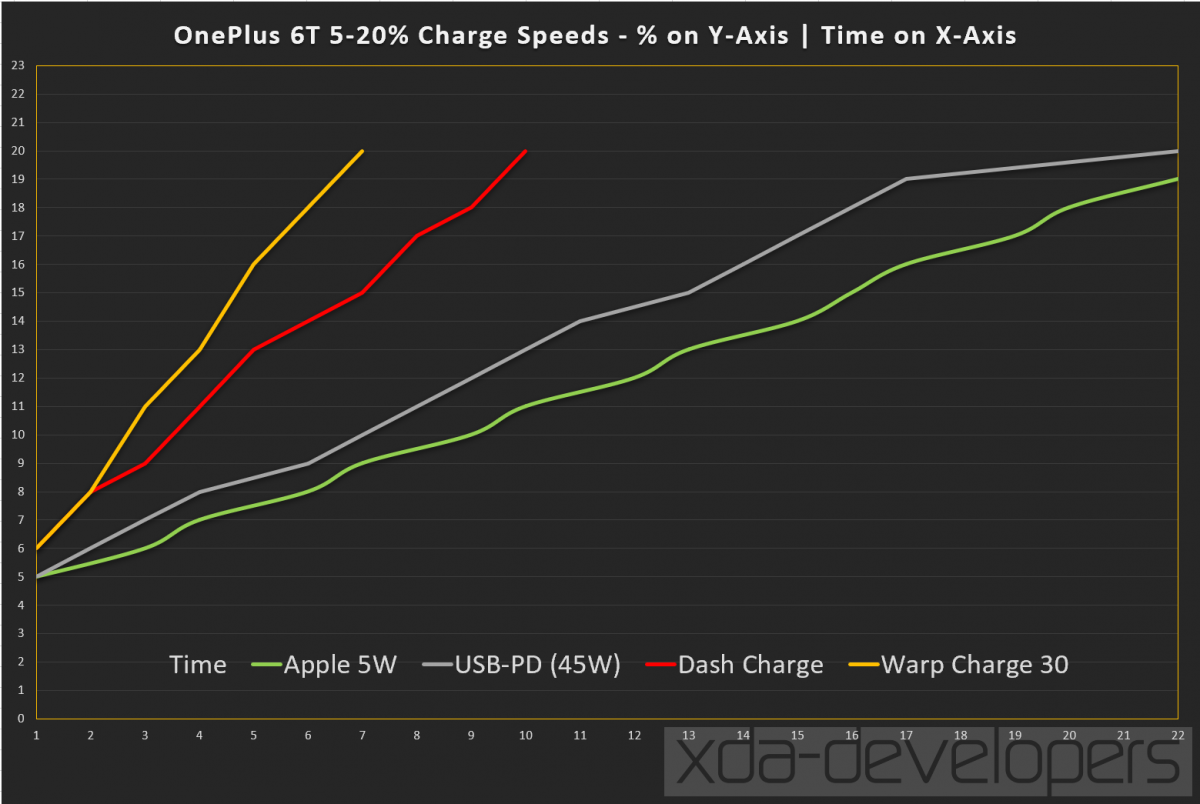
\includegraphics[width=\linewidth]{images/image13}
  \caption{OnePlus 6T charge speeds from 5-20\% using Apple 5W, Dash Charge, WARP chargers respectively and USB-Power Delivery\cite{b18}}
\end{figure}

The above Fig.13 shows us the use of different standards and equipment on a WARP charge supported device. It is observed that WARP charge charges faster than others.

One of the main benefits of Warp Charge is its ability to keep temperatures low while charging. The fast charging option allows you to watch videos or play games while the phone is charging, with no net drop in charging speeds. That isn't the case with Quick Charge, as the higher voltages invariably lead to the phone reverting to normal speeds to prevent overheating\cite{b17}. WARP supported phone can charge up to 50\% in just 20 minutes, it takes an additional 40 minutes to fully charge the battery. That's to prevent damage to the battery (and more importantly, you), with the wall charger limiting output at 2A after hitting 75\% and going even lower after reaching 85\%. The micro controller unit inside the phone constantly monitors the charge level to determine the desired amperage to be delivered\cite{b17}.

The facts posted by the OEM was backed by a real tester in a test by Mr. Daniel Marchena and results were posted back in a comprehensive comparison post \cite{b18}. 

\begin{figure}[h!]
  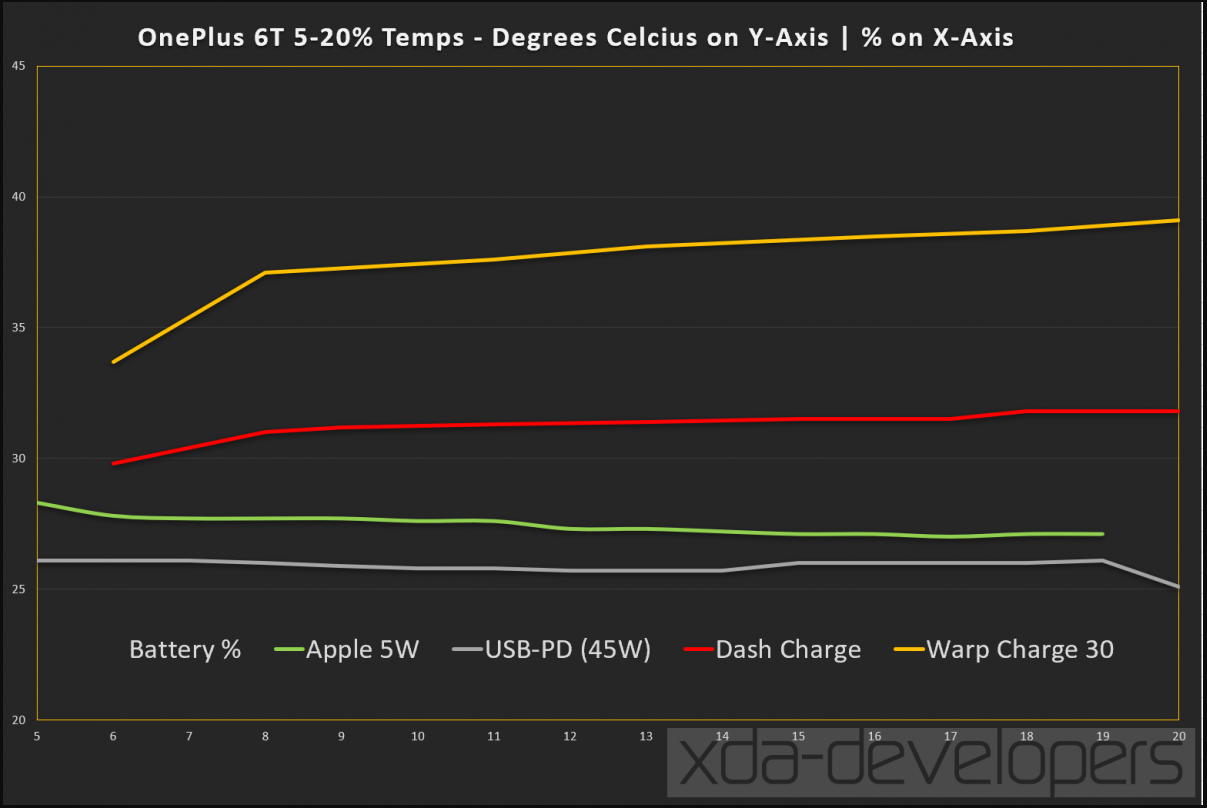
\includegraphics[width=\linewidth]{images/image14.png}
  \caption{ Temperature scale for OnePlus 6T 5-20\% \cite{b18}}
\end{figure}

In the above Fig.14 Temperature Scale is seen with use of different chargers for the same scenario as Fig.13.

\section{Discussion}

To start with the discussion, the most important point of this Thesis is to show how charging is affected while using your device. This results into slow charging speeds and also might affect performance of device. Different charging schemes discussed above have various offerings and better over each other. However, WARP Charge 30 seems to edge past AQC and Dash Charge with some benifts of its own. One of the main benefits of Warp Charge is its ability to keep temperatures low while charging. The fast charging option allows you to watch videos or play games while the phone is charging, with no net drop in charging speeds. That isn't the case with Quick Charge, as the higher voltages invariably lead to the phone reverting to normal speeds to prevent overheating\cite{b17}. Some devices have been known in the past to actually turn off Fast Charging support while the display is on, and some remain to a trickle charge, not to mention heavy usage such as Gaming. 

\begin{figure}[h!]
  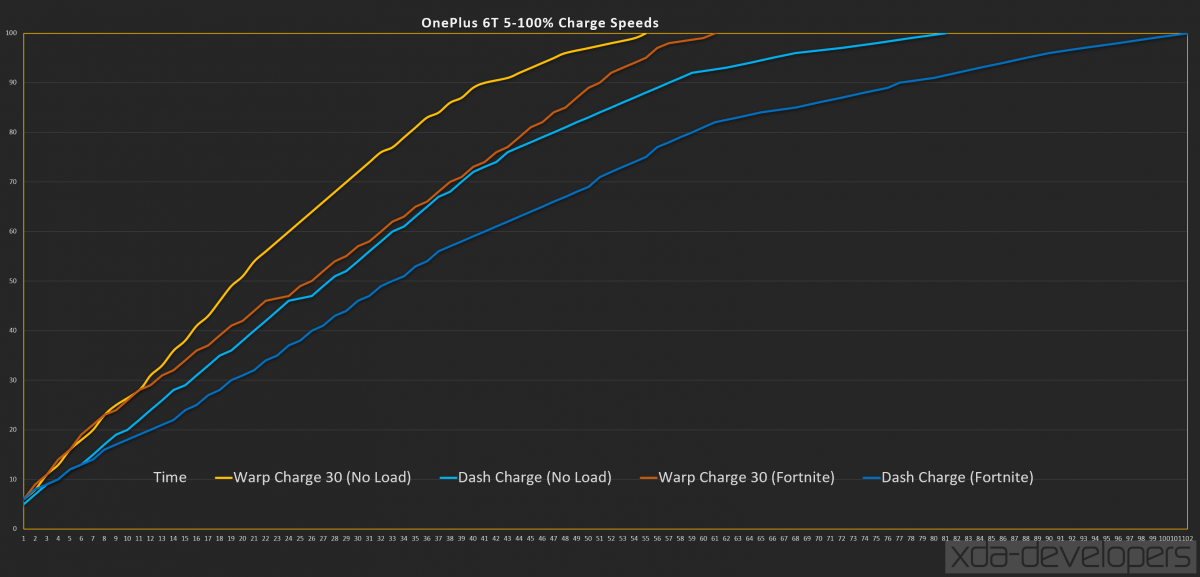
\includegraphics[width=\linewidth]{images/image15.png}
  \caption{ Warp Charge 30 vs Dash Charge with Baseline and Load\cite{b18}}
\end{figure}

While the bench-marking and testing, the author\cite{b17} drained the device to 5\% battery, waited until it cooled down and the plugged it in once it was already loaded into a match of Fortnite(Mobile Game). Then performed a baseline for both Dash Charge as well as Warp Charge 30 to see how differently the OnePlus 6T McLaren Edition performed\cite{b18}. 

Here is how the McLaren Edition OnePlus 6T reacts under load and this is where things get a little interesting. Warp Charge 30 is significantly faster than Dash Charge while gaming, and behaves differently too. It was observed that 5\%-100\% benchmark took only 60 minutes – a mere 6 minutes longer than baseline no load test – and crushed the Dash Charge which took a, by comparison, long 81 minutes to fully charge without load, and 101 minutes under load. Peering deeper into the data there were some significant things. The first is that Warp Charge 30 loves to cram power in quickly, but it is cautious of the overall battery temperature. Right at about 19\% battery we see Warp Charge 30 drastically drop the current coming into the device and at this same time the battery hit 44 degrees Celsius. It did not get back to over 3,000 mA of Current for a bit when the battery temp was back in check. Looking at baseline non-load numbers, you can see where the tiers of charging power are in Warp Charge 30. It is not until the battery is at 25\% charge that has seen a significant drop in current into the device of about 500mA and then again at 35\%  then it drops another 1,000mA. From there it drops slowly but steadily until it hits its final drop around 80\% charge. This is in contrast to the curve the Dash Charger had. The Dash Charger will stay fairly constant until it hits 70\% charge, where it will throttle back the current by about half and is why their graph curves fall off right around that range\cite{b18}. 

\begin{figure}[h!]
  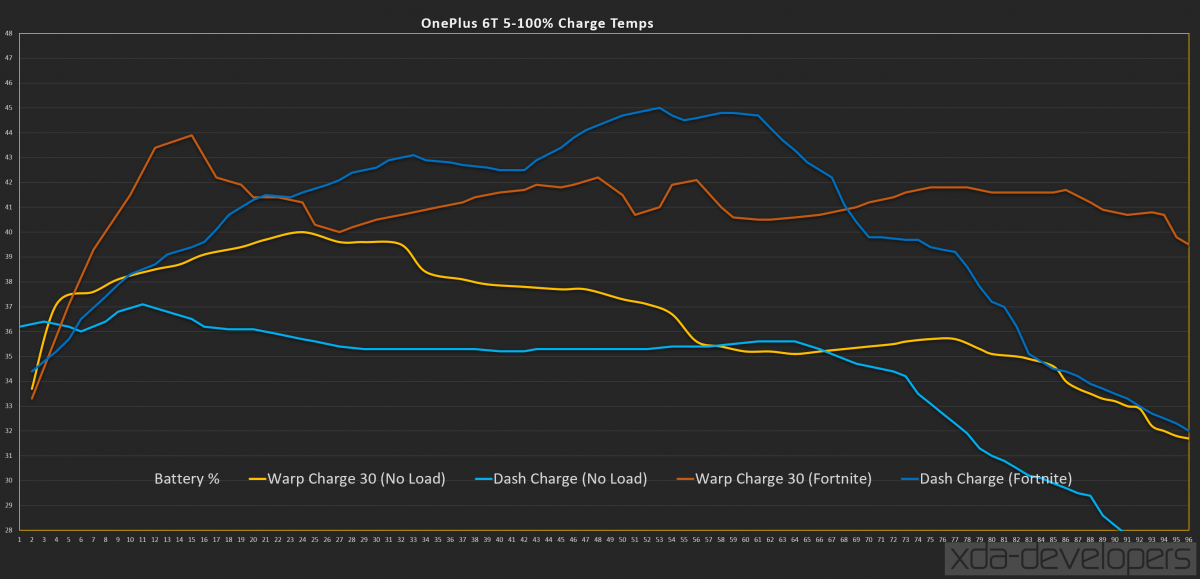
\includegraphics[width=\linewidth]{images/image16.png}
  \caption{ Temperature observation while using device vs while gaming in Dash and Warp respectively.\cite{b18}}
\end{figure}

In terms of temperatures, there is not a huge difference between Dash and Warp Charge 30 here, but there is higher across the board in most cases. The largest gap is around 10\% battery where the Warp Charge 30 has the battery about 5 degrees warmer. That is until it has that drop in current that is discussed above and from there they run similarly with Warp Charge 30 actually staying cooler than Dash Charge under load until we hit 70\% battery. Around 75\% battery, the Dash Charge falls flat dropping from 2,300 mA down to 1,000 mA and sometimes lower. This behavior is also present on the OnePlus 6 with the Dash Charge, so it is likely by design and not something at fault which is likely the wise move to preserve battery longevity\cite{b18}.


\section{Conclusion}

After deep understanding of different concepts related to various fast charging schemes available in smartphones, it was seen that every charging schemes have their own pros and cons. This is because of various specifications and underlying hardware used by the OEMs. With the study of this thesis we can also learn that the closest competitors were Warp and Dash Charge schemes implemented by the OEM. Warp Charge 30 is excellent, especially if you like to game or do heavy usage while charging. Just like Dash Charge, a customer can own a device that runs cooler than most others while charging, and gain battery even while pushing the device with one of the more demanding and popular titles. Temperatures are also becoming more of an issue here as well. While it still needs to look to having a proper comparison with other devices on the market, Warp Charge 30 still runs cool while under load and charging but it is a not-so-insignificant bump of around 20\% warmer in our 5\%-20\% charging test versus Dash Charge. While gaming though, the device is only 14\% warmer than baseline results which is a really solid result considering much of that heat likely comes from the SoC(System on Chip). Conservatively it was found that a 10\%-15\% bump in battery temps using Warp Charge 30. While this charger does not seem to generate the level of heat as seen from other charging solutions, Warp Charge 30 in a no-load scenario still runs warmer than Dash Charge under load. But again it comes down to the hardware and software tweaks applied by the manufacturers which make their products attractive and advanced then the others competing. To conclude this thesis, fast/rapid charging standards will be improving day by day, bringing more parameters into consideration along with their architecture which will play a big role in future work. 



\begin{thebibliography}{00}
\bibitem{b1} M. D. Kim, M. S. Jeon, M. S. Lee, and H. Cha, “Always-On Quick Charging for Mobile Devices,” IEEE International Conference on Pervasive Computing and Communications, p. 10, 2019.
\bibitem{b2} L. He, E. Kim, and K. G. Shin, “*-Aware charging of lithium-ion battery cells,” in Proceedings of the 7th International Conference on CyberPhysical Systems, 2016, p. 26: IEEE Press.
\bibitem{b3} L. He, Y.-C. Tung, and K. G. Shin, “iCharge: User-Interactive Charging of Mobile Devices,” in Proceedings of the 15th Annual International Conference on Mobile Systems, Applications, and Services  - MobiSys ’17, Niagara Falls, New York, USA, 2017, pp. 413–426.
\bibitem{b4} Qualcomm Quick charge, https://www.qualcomm.com/solutions/mobile
computing/features/quick-charge, [Online; accessed June 2019] 
\bibitem{b5} Fast Adaptive Charging, http://www.samsung.com/global/galaxy/whatis
/adaptive-fast-charging/, [Online; accessed June 2019]
\bibitem{b6} Dash Charge, https://www.oneplus.com/uk/dashcharge [Online; accessed June 2019]
\bibitem{b7} K. Zaghib et al., “Safe and fast-charging Li-ion battery with long shelf life for power applications,” Journal of Power Sources, vol. 196, no. 8, pp. 3949-3954, 2011. 
\bibitem{b8} L.-R. Chen, R. C. Hsu, and C.-S. Liu, “A design of a grey-predicted Li ion battery charge system, ”IEEE Transactions on Industrial Electronics, vol. 55, no. 10, pp. 3692-3701, 2008
\bibitem{b9} L. He, E. Kim, and K. G. Shin, “*-Aware charging of lithium-ion battery cells,” in Proceedings of the 7th International Conference on CyberPhysical Systems, 2016, p. 26: IEEE Press. 
\bibitem{b10} G. Bhat, S. Gumussoy, and U. Y. Ogras, “Power-temperature stability and safety analysis for multiprocessor systems,” ACM Transactions on Embedded Computing Systems (TECS), vol. 16, no. 5s, p. 145, 2017.
\bibitem{b11} Q. Xie, J. Kim, Y. Wang, D. Shin, N. Chang, and M. Pedram, : “Dynamic thermal management in mobile devices considering the thermal coupling between battery and application processor,” in Computer-Aided Design(ICCAD), 2013 IEEE/ACM International Conference on, 2013, pp. 242-247: IEEE. 
\bibitem{b12} R. Muralidhar et al., “Experiences with power management enabling on the Intel Medfield phone,” in Proc. of Linux Symposium, 2012, pp. 35-46. 
\bibitem{b13} Blog Article by Robert Triggs., “How fast charging really works,” Android Authority,30-Jan-2019. [Online]. Available:
https://www.androidauthority.com/fast-charging-explained-889780/. 
[Accessed: June 2019].
\bibitem{b14} Wikipedia-VOOC, https://en.wikipedia.org/wiki/VOOC\#cite\_note-onep-5 Wikipedia. 01-Jul-2019.
\bibitem{b15} “OPPO VOOC Flash Charge takes on Qualcomm’s Quick Charge 2.0,” Android Authority, 26-Mar-2015. [Online]. Available: https://www.androidauthority.com/oppo-vooc-flash-charge-596939/. [Accessed: 25-Jul-2019].
\bibitem{b16} “What is the OnePlus 3 DASH charging/sync cable doing internally?? Let’s probe it!,” OnePlus Community. [Online]. Available:
https://forums.oneplus.com/threads/what-is-the-oneplus-3-dash-charging-sync-cable-doing-internally-lets-probe-it.456017/. [Accessed: Jul-2019].
\bibitem{b17} “All you need to know about OnePlus’ 30W Warp Charge standard,” Android Central, 24-May-2019. [Online]. Available: https://www.androidcentral.com/warp-charge. [Accessed: Jul-2019].
\bibitem{b18} “Warp Charge 30 on the OnePlus 6T McLaren Edition is Fast and Cool,” xda-developers, 13-Dec-2018. [Accessed: Jul-2019].




\end{thebibliography}
\vspace{12pt}

\end{document}
